% Copyright (C) 2012 Thomas L. Kula
% All Rights Reserved
%
% See the file LICENSE for license terms.
\documentclass[12pt]{article}
\usepackage{graphicx}
\usepackage{rotating}
\usepackage{fix-cm}
\usepackage{multirow}
\setlength{\paperwidth}{5.5in}
\setlength{\paperheight}{8.5in}
\setlength{\textheight}{7.45in}
\setlength{\topmargin}{-1.0in}
\setlength{\oddsidemargin}{-0.5in}
\setlength{\evensidemargin}{-0.5in}
\setlength{\textwidth}{4.0in}
\setlength{\parindent}{0in}
\setlength{\parskip}{3mm}
\usepackage[print]{booklet} \nofiles
\source{\magstep0}{5.5in}{8.5in}
\target{\magstep0}{11in}{8.5in}
\setpdftargetpages
\pagestyle{empty}
\begin{document}


\begin{center}
{\fontsize{36}{48}\selectfont \textsc{Haiku a Day }}
\end{center}

\vspace*{3.5cm}

{\fontsize{20}{40}\selectfont 

Summer, drawing close

Nudges the shoulder of Spring

Whispering, ``my turn''


}

\vspace*{5.0cm}
\begin{center}
{\large{Issue 82: April 2012}} \\[5mm]
{\fontsize{8}{8}\selectfont  \textsc{ St. Joshua Norton Press }} \\[1mm]
{\fontsize{6}{6}\selectfont Mathom House by the Cloisters \textbar The People's Republic of Ames }
\end{center}


\newpage



--- Thomas

http://kula.tproa.net/had/ \\
kula@tproa.net

Download this and previous HADs at the website, so you can
print out your own (DIY, yeah!) or if you want me to send
you one, send me your address, and maybe a stamp if you
are feeling nice. Or send me something you've made ---
trades always appreciated, postcards are nice too.

\vfill

1 April 2012

When the sunny days \\
Turn one's thoughts to summer time \\
And grilling parties

2 April 2012

One does not simply \\
Walk calmly into Mordor --- \\
There's a ticket booth

\newpage

3 April 2012

Double-secret? Hah! \\
Triple-secret probation \\
Is what you suffer

4 April 2012

Into a bar walk \\
Gatekeeper and Keymaster --- \\
Barkeep crosses streams

5 April 2012

Save the orphanage \\
Requires a car chase of \\
Epic proportions

6 April 2012

The list continues: \\
The sixteenth rule of Fight Club: \\
Tuesday night: tacos

7 April 2012

A fresh rain washes \\
Making the streets look pretty \\
--- maybe an hour

8 April 2012 

Useless bookcases: \\
Speakers I no longer use \\
Hold a stack of books 

9 April 2012

Motorcyclists: \\
Most of them I'm fine with, \\
Asshole ones I hate

\newpage

10 April 2012

Soft bean curd wallows \\
A fluffy cloud, salty sauce; \\
Tempura crunches

11 April 2012

Ominous clicking \\
From the radiator pipes \\
It stops suddenly

12 April 2012

Apartment hydra \\
A mess of cables growing \\
Knotting, and waiting

13 April 2012

Perambulating \\
Is the finest therapy \\
For a cool spring day

14 April 2012

It's $\pi + 1$ day \\
Any old excuse for pie \\
Is good in my book

15 April 2012

Dammit, now I want \\
Pie --- yesterday was kidding \\
Today it is real

16 April 2012

Where is the Thai food? \\
Why can't we find the Thai food? \\
We walked right past it.

\newpage

17 April 2012

How can just one week \\
Turn a pretty park from plain \\
To lushly verdant?

18 April 2012

Brain stuck on fire \\
Then the afternoon fizzle \\
Blank stare an hour

19 April 2012

There are scissors here \\
I know I packed at least three \\
So where are they now?

20 April 2012

I need poster frames \\
And the abundance of choice \\
Is locking my brain

21 April 2012

Windows need cleaning \\
Which would seem to require \\
Rocket boots or such

22 April 2012

Bloop bloop bloop bloop bloop \\
My brain is not on today \\
So you get this junk

23 April 2012

Full of cells growing \\
Living, dying, dividing \\
Just freaking me out

\newpage

24 April 2012

The flutter of birds \\
Quiet, peaceful and calming. \\
Not at five a.m.

25 April 2012

Why must you taunt me \\
Sugar roasted peanut guy? \\
You torture my day.

26 April 2012

When I am busy \\
The time for library books \\
Passes too quickly

27 April 2012

Slow, majestically \\
The {\em Enterprise} passes by \\
It's soon to be home

28 April 2012

The lure of pizza \\
Ever is my nemesis \\
Someday I will beat

29 April 2012

Why do I keep this? \\
It's a recipt: months ago \\
I bought groceries

30 April 2012

Is it a cliche \\
To wonder where the month went? \\
It happens often.

\newpage

\begin{center}
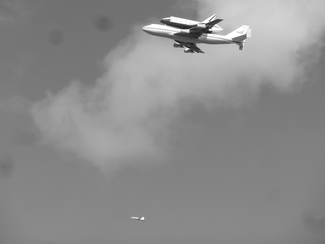
\includegraphics[width=325pt]{enterprise.png}

The Space Shuttle Enterprise (OV-101) atop the Shuttle Carrier Aircraft 
flies past the USS Intrepid Museum accompanied by a NASA T-38 Trainer  \\
27 April 2012 \\
{\tt http://kula.tproa.net/photos/2012/20120427-enterprise/}
\end{center}

\newpage

\thispagestyle{empty}
\vspace*{12cm}
\begin{sideways}
\Large{St. Joshua Norton Press}
\end{sideways}
\begin{sideways}
\Large{PO Box 250138}
\end{sideways}
\begin{sideways}
\Large{New York NY 10025}
\end{sideways}


\end{document}


